\documentclass[11pt]{article}
\usepackage[utf8]{inputenc}
\usepackage{amsmath, amssymb}
\usepackage{graphicx}
\usepackage{hyperref}
\usepackage{geometry}
\geometry{margin=1in}

\title{Expanding Entropy and the Birth of Spacetime}
\author{Juha Meskanen}
\date{2018}

\begin{document}
\maketitle


\begin{abstract}
   We explore the hypothesis that the growth of entropy in a computable execution trace corresponds to the expansion of spacetime,
   offering a natural explanation for the low-entropy initial state of the universe and its inflationary growth. Using simple simulations
   based on bit string evolution and particle definitions from minimal structures, we demonstrate that entropy
   increase drives an emergent geometric expansion. Furthermore, we uncover that the statistical distribution of emergent
   structure probability follows a lognormal pattern.
\end{abstract}

\section{Introduction}

Why did the universe begin in such a finely tuned state? And why does entropy continue to increase as the universe expands?
These questions have often been treated as separate, but we argue that they are fundamentally linked.
In our previous work, we proposed an information-theoretic framework to describe the collapse of spacetime geometry through
the lens of entropy reduction, formalized in the **Entropy-Singularity Lemma**: *vanishing entropy implies geometric
singularity* \cite{Paper1}.

In this paper, we reverse this process, postulating that the **increase in entropy** corresponds to the expansion of spacetime,
effectively mapping the increase in informational complexity to cosmological expansion.


\section{Entropy as a Driver of Expansion}

We define an execution trace ${S_t}_{t=0}^n$, where each $S_t$ is a binary string of fixed length $L$.
Starting from a state of zero entropy (all-zero string), we evolve $S_t$ forward using a random bit-flip mutation process that
incrementally increases entropy.

Each $S_t$ is interpreted geometrically through a decoding scheme $D: \{0,1\}^L \to \mathbb{R}^d$. In this study,
we define the hierarchy of elementary structures as follows:

1. **Spacetime fabric:** Directly defined by 3D points encoded from the bistrings through the decoding scheme.

2. **Elementary Particles:** These are defined as pairs of 3D points, i.e., pairs of
coordinates $((x_1, y_1, z_1), (x_2, y_2, z_2))$, where the spatial separation between the
points is fixed. Specifically, an elementary particle is formed when two points in the 3D space are within
a certain threshold distance, indicating that they can be considered a pair of interacting points.

3. **Atoms:** We define an atom as a set of three points $(p_1, p_2, p_3)$ where the distances between the points satisfy:
\[
   0 < \text{distance}(p_1, p_2) < \text{threshold}, \quad 0 < \text{distance}(p_2, p_3) < \text{threshold}, \quad 0 < \text{distance}(p_3, p_1) < \text{threshold},
\]
and the distances are sufficiently close to each other such that the structure is nearly equilateral

4. **Molecules:** A molecule is formed when two atoms are sufficiently close in space, with the distance between
their centers being below a given threshold. The center of an atom is defined as the geometric center of the three points forming the atom:
\[
   \text{center}(atom) = \left( \frac{x_1 + x_2 + x_3}{3}, \frac{y_1 + y_2 + y_3}{3}, \frac{z_1 + z_2 + z_3}{3}, \frac{t_1 + t_2 + t_3}{3} \right).
\]
A molecule is considered to be formed when the distance between the centers of two atoms, $atom_1$ and $atom_2$, is below a threshold value:
\[
   \text{distance}(\text{center}(atom_1), \text{center}(atom_2)) < \text{threshold}.
\]
Thus, a molecule is a structure consisting of two atoms in close proximity, representing the next level of complexity in the hierarchy.


We define a decoding rule that extracts these particles from substrings of $S_t$, and count the number of distinct particles
present at each timestep. We simulate the evolution of $S_t$ by applying random bit flips, which increase the Shannon entropy of the string.
We find:

\begin{enumerate}
   \item Initially, when entropy is near zero, no valid particles are decoded.
   \item As entropy increases, particle count grows exponentially.
   \item This exponential rise slows as entropy increases further, matching the inflationary burst followed by slower expansion.
\end{enumerate}



\section{Statistical Properties: Lognormal Emergence}

Plotting the number of valid geometric interpretations (particles, atoms, molecules) against entropy yields a distribution resembling a lognormal curve.  The results also show that at lower entropy, only elementary particles exist, while at higher entropy, atoms and molecules emerge. This aligns with observed cosmic evolution: inflation (early burst), structure formation, and degeneration during late-time hen the entropy reaches its maximum. The simulation also demonstrate natural progression from simple to complex forms as entropy increases.

\begin{figure}[h!]
   \centering
   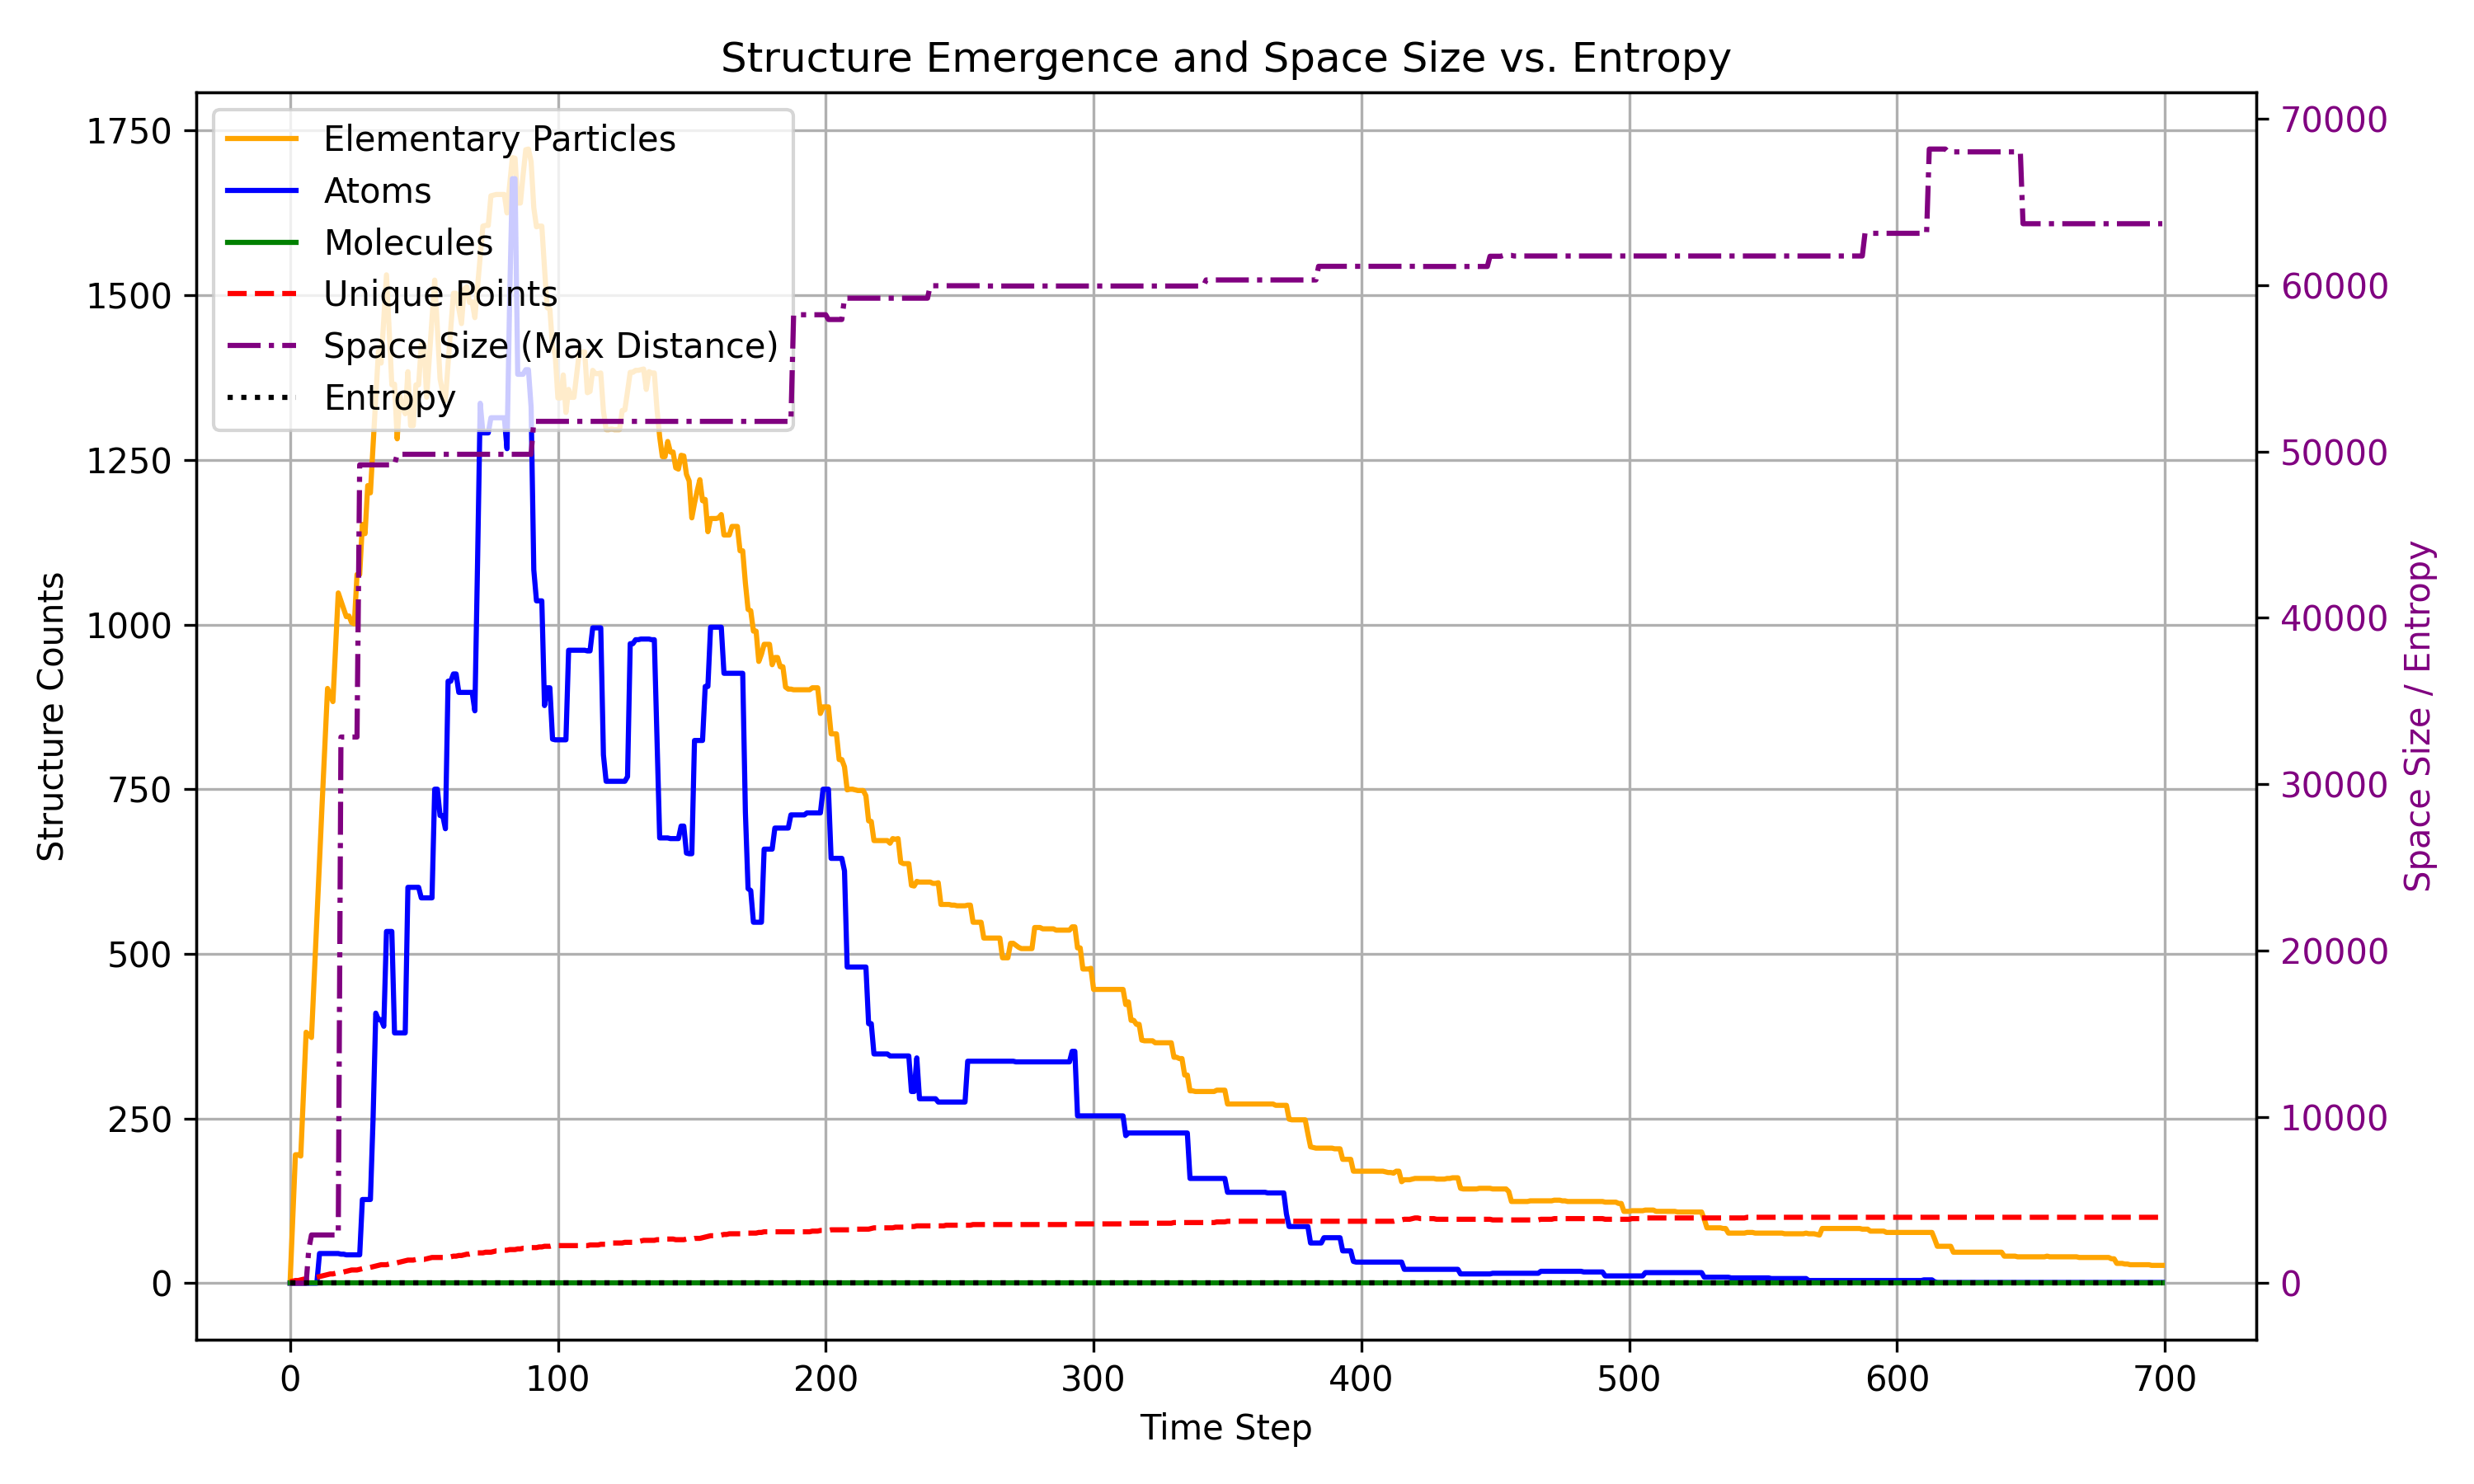
\includegraphics[width=0.8\textwidth]{figures/entropy_to_matter.png}
   \caption{Emergence of hierarchical structures in the execution trace. The emergence follows a lognormal-like distribution.}
   \label{fig:lognormal-structure}
\end{figure}

The simulation program is hosted at \url{http://github.com/juhakm/emergence_of_spacetime.py}.


\section*{Implications for Spacetime Geometry}

Despite its minimal assumptions and lack of conventional predictive machinery, our model reveals consistent structural patterns in the evolution of bitstring-based universes. One of the most striking observations is the emergence of a lognormal distribution in the frequency of microstructures as entropy increases from its minimum.

This statistical regularity has direct geometric implications: it suggests that the probability of matter — interpreted here as persistent, compressible patterns — is correlated with entropy. Near the entropy minimum, where the informational configuration consists of long, uniform bitstrings (e.g., all 0s or 1s), the probability of finding any distinguishable structure approaches zero. Without structure, there is no particle content — and therefore, no gravity.

This leads to a provocative conclusion: the curvature of spacetime at the singularity is not infinite, as predicted by General Relativity, but zero. The singularity, in this view, is not a region of divergent geometry but a trivial state.

This interpretation stands in stark contrast to both General Relativity, which predicts infinite curvature at the singularity, and Quantum Mechanics, which typically excludes the possibility of a fully defined, zero-entropy state. Yet, in our simulation, the universe begins in precisely such a state, and coherent geometric structures emerge only as entropy increases.


\section{Future Work}

This paper establishes a computational framework in which entropy increase corresponds to the emergence of spacetime geometry and structure, offering a clean statistical alternative to the singular initial conditions postulated by General Relativity and Quantum Mechanics.

We will explore the implications of the observed breakdown of both GR (due to singularities) and QM (due to the assumption of nonzero entropy at origin), and construct a unified information-theoretic framework to describe phenomena attributed to spacetime curvature and quantum entanglement.

Ultimately, we aim to replace geometric and probabilistic descriptions of the universe with a single, consistent, fully self-contained model that expect no substrace beyond information itself.


\end{document}

